\documentclass{scrartcl}

\RequirePackage{amsmath, amssymb, url, microtype,xcolor}
\usepackage{mathtools}
% \usepackage{palatino}
%\usepackage{euler}

\usepackage{mathdots}
\usepackage[amsmath,thmmarks]{ntheorem}
\usepackage{thmtools}%for nameref to work right
\usepackage{nameref}
\usepackage[colorlinks=true,linkcolor=blue,citecolor=blue,urlcolor=blue]{hyperref}
\usepackage{cleveref}
\renewcommand{\ref}{\hyperref}
\newcommand{\nameclevref}[1]{\nameref{#1} (\cref{#1})}
\usepackage{microtype}
\usepackage[draft,rivers]{impnattypo}

\newtheorem{theorem}{\normalfont\sffamily{}Theorem}

\providecommand{\Z}{\mathbb{Z}}
\providecommand{\N}{\mathbb{N}}
\providecommand{\R}{\mathbb{R}}
\providecommand{\C}{\mathbb{C}}
\providecommand{\Q}{\mathbb{Q}}
\providecommand{\id}{\mathrm{id}}

% proof environment
\makeatletter
\newcommand{\openbox}{\leavevmode
  \hbox to.77778em{%
  \hfil\vrule
  \vbox to.675em{\hrule width.6em\vfil\hrule}%
  \vrule\hfil}}
\gdef\proofSymbol{\openbox}
\newcommand{\proofname}{\color[gray]{.3}\normalfont\sffamily{}Proof.}
\newcounter{proof}\newcounter{currproofctr}\newcounter{endproofctr}%
\newenvironment{proof}[1][\proofname]{
  \th@nonumberplain
  %\def\theorem@headerfont{\sffamily}%
  \normalfont
  \theoremsymbol{\ensuremath{_\blacksquare}}
  \@thm{proof}{proof}{#1}}%
  {\@endtheorem}
\makeatother

\usepackage{fontspec}
\setmainfont[Ligatures={Common,Required,TeX},Numbers=OldStyle]{Linux Libertine O}
\setsansfont[Numbers=OldStyle,Ligatures={Common,Required,TeX}]{Linux Biolinum O}

\usepackage[euler-digits,euler-hat-accent,small]{eulervm}

% \newcommand{\mathbold}{\mathbf}
\renewcommand{\vec}{\mathbold}
\newcommand{\f}{\vec f}

\setkomafont{section}{\Huge\normalfont\sffamily\color[gray]{.5}}
\setkomafont{subsection}{\Large\normalfont\sffamily\color[gray]{.3}}
\setkomafont{subsubsection}{\large\normalfont\sffamily\color[gray]{.2}}

\renewcommand{\labelitemi}{\color[gray]{.5}\textbullet}
\title{\normalfont\sffamily\color{darkgray} The derivative matrix}
\author{Riley Levy}
\begin{document}
\maketitle
\section{Vectors}
A $n$-dimensional vector is an ordered pair of $n$ real numbers. This is written
as
\[
  (x,y,z,\dots,\omega)=
  \begin{bmatrix}
    x \\ y \\ z \\ \vdots \\ \omega
  \end{bmatrix}
\]
The space $\R^n$ of ordered real $n$-tuples is called the $n$-dimensional vector space.
Vectors will be written in boldface: $\vec x$, matrices will be written as
capitals: $A$, scalars will be written plainly: $k$.

Vectors are added by
\[
  (x_1,x_2,\dots,x_n)+(y_1,y_2,\dots y_n) = (x_1+y_1, x_2+y_2, \dots, x_n+y_n)
\]
or written as column vectors is a special case of matrix addition
\[
  \begin{bmatrix}x_1 \\ x_2 \\ \vdots \\ x_n\end{bmatrix}+
  \begin{bmatrix}
    y_1 \\ y_2 \\ \vdots \\y_n
  \end{bmatrix}
  =
  \begin{bmatrix}
    x_1+y_1 \\ x_2+y_2 \\ \vdots \\ x_n+y_n
  \end{bmatrix}
\]
You can ``scale'' or ``scalar multiply'' a vector via
\[
  k(\vec x_1,\vec x_2,\dots \vec x_n)=(k\vec x_1,k\vec x_2,\dots k\vec x_n)
\]
Geometrically, this stretches or compresses the vector by a factor of $k$, where
$k$ is a real number

You can combine vectors and scalars to get a new vector using these operations.
This is called a linear combination. Formally, a linear combination of the
vectors $\vec x_1,\dots, \vec x_n$ is
\[
  a_1\vec x_1+a_2\vec x_2+\dots + a_n\vec x_n
\]
\newcommand{\basis}{\vec e}
The standard basis of $\R^n$ is the set of vectors
\[
  \basis_1=
  \begin{bmatrix}
    1 \\ 0 \\ \vdots \\ 0
  \end{bmatrix},
  \basis_2=
  \begin{bmatrix}
    0 \\ 1 \\ \vdots \\ 0
  \end{bmatrix},\dots
  \basis_n=
  \begin{bmatrix}
    0 \\ 0 \\ \vdots \\ 1
  \end{bmatrix}
\]
Any vector in $\R^n$ can be written as a unique linear combination of the
standard basis vectors. Consider the example
\[
  (a,b,c)=a\basis_1+b\basis_2+c\basis_3
\]

Define the dot product of two vectors by
\[
  (x_1,x_2,\dots x_n)\cdot (y_1,y_2,\dots y_2)=x_1y_1+x_2y_2+\dots x_ny_n
\]
Note the length of $\vec x$, $|\vec x|=\vec x \cdot \vec x$.

A function $\f=(f_1,f_2,\dots f_n)$ has derivative
\[
  \f'=(f_1',f_2',\dots f_n')
\]
\subsection*{Problems}
\begin{enumerate}
\item The function $t\mapsto (\cos t, \sin t)$ traces a unit circle with unit
  speed. Use the fact the tangent to a circle is perpendicular to the radius to
  show $\sin'=\cos$ and $\cos'=-\sin$
\item Derive the centripital acceleration of a particle moving in a circle of
  radius $r$ with angular velocity $\omega$. Its position as a function of time is
  \[
    t\mapsto r(\cos \omega t, \sin \omega t)
  \]
\end{enumerate}
\section{Linear functions}
A function $\f$ is said to be linear iff
\begin{itemize}
\item $\f$ distributes over vector addition:
  \[
    \f(\vec x+ \vec y)=\f(\vec x)+\f(\vec y)
  \]
\item $\f$ commutes with scalar multiplication
  \[
    \f(k\vec x)=k\f(\vec x)
  \]
\end{itemize}
equivalently, $f$ is linear iff it preserves linear
combinations:
\[
  \f(a_1\vec x_1 + a_2 \vec x_2 + \dots + a_n \vec x_n) = a_1\f(\vec x_1) + a_2 \f(\vec x_2) + \dots + a_n \f(\vec x_n)
\]

It's not obvious yet but this is the generalization needed to make ``local
linearity'' or ``best linear approximation'' meaningful in higher dimensions,
which we use to make sense of the derivative.

Some examples of linear maps are:
\begin{itemize}
\item scalar multiplication
\item matrix multiplication
\item rotations and dilations centered at the origin
\item reflections in lines through the origin
\item even $d/dx$ and $\int$ are linear in some sense: they
  commute with constant multiplication and distribute over addition.
\end{itemize}

\section{Matrices}
Matrices are essentially coordinate representations for linear maps (in finite
dimensional spaces).

Here's a diagram of matrix multiplication:

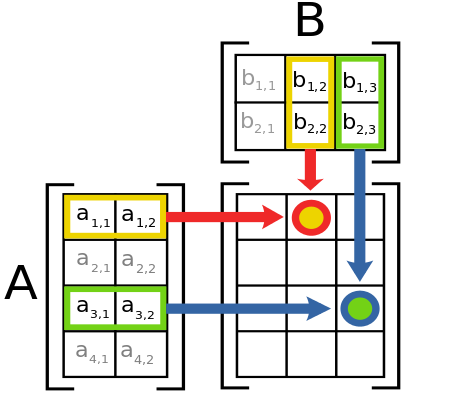
\includegraphics[width=\textwidth]{matrix-mult.png}

Matrix multiplication goes row dot-product column. So the red/yellow circle will
have the value $(AB)_{12}=a_1\cdot b_1$. The green/blue circle has value
$(AB)_{33}=a_{31}b_{13}+a_{32}b_{23}$.

In general,
\[
(AB)_{ij}=\sum_{k} a_{ik}b_{kj}
\]
The dot product is a special case of matrix multiplication:
\[
  \vec x\cdot \vec y=\vec x^\top \vec y
\]
where $\vec x^\top$ is the \emph{transpose} of $\vec x$:
\[
  \begin{bmatrix}
    x_1 \\ x_2 \\ \vdots \\ x_n
  \end{bmatrix}^\top
  =
  \begin{bmatrix}
    x_1 & x_2 & \dots & x_n
  \end{bmatrix}
\]
In general,
\[
  \begin{bmatrix}
    a & b \\ c & d
  \end{bmatrix}^\top =
  \begin{bmatrix}
    a & c \\ b & d
  \end{bmatrix}
\]

The matrix
\[
  I =
  \begin{bmatrix}
    1 & 0 & 0 &\dots& 0 \\
    0 & 1 & 0 &\dots& 0 \\
    0 & 0 & 1 &\dots& 0 \\
    \vdots & \vdots & \vdots & \ddots & \vdots\\
    0 & 0 & 0 & \dots & 1
  \end{bmatrix}
\]
is called the identity matrix. It is the multiplicative identity for matrices:
\[
  xI=Ix=x
\]
\subsubsection*{Problems}
A square matrix $M$ has an inverse if there is some matrix $M^{-1}$ such that
\[
  MM^{-1}=M^{-1}M = I
\]
\begin{enumerate}
  \item
    Show by multiplying with $
\begin{bmatrix}
  a & b \\ c & d
\end{bmatrix}$
the following do not have inverses:
  $ \begin{bmatrix}
      1 & 0 \\ 0 & 0
    \end{bmatrix} $,
    $\begin{bmatrix}
      1 & 1 \\ 0 & 0
    \end{bmatrix}
    $,
  $
    \begin{bmatrix}
      1 & 0 \\ 1 & 0
    \end{bmatrix}
    $,
    $
    \begin{bmatrix}
      1 & 1 \\ 1 & 1
    \end{bmatrix} $.
  \item \label{complex-as-matrix}
    Show you can represent complex numbers with the encoding
  \begin{align*}
   1 &\mapsto
       \begin{bmatrix}
         1 & 0\\ 0 & 1
       \end{bmatrix}
\\
    i&\mapsto \begin{bmatrix} 0 & -1 \\ 1 & 0 \end{bmatrix}
  \end{align*}
   More explicitly,
  \[
    (a+bi)(c+di)\mapsto\left (a
    \begin{bmatrix}
     1 & 0 \\ 0 & 1
    \end{bmatrix}
    + b
    \begin{bmatrix}
      0 & -1 \\ 1 & 0
    \end{bmatrix} \right)
  \left(c
     \begin{bmatrix}
     1 & 0 \\ 0 & 1
    \end{bmatrix}
    + d
    \begin{bmatrix}
      0 & -1 \\ 1 & 0
    \end{bmatrix}
  \right)
  \]
  gives the correct product.
  (Hint: Note
  $\left[\begin{smallmatrix}
    1 & 0 \\ 0 & 1
  \end{smallmatrix}\right]$
  is the identity matrix. Then it suffices to show
  $\left[
  \begin{smallmatrix}
    0 & -1 \\ 1 & 0
  \end{smallmatrix}  \right]^2 = -I
  $. The rest follows by linearity.)
\item Matrix multiplication is not commutative in general. Check that
  \[
    \begin{bmatrix}
      1 & 0 \\ 0 &0
    \end{bmatrix}
    \begin{bmatrix}
      0 & 1 \\ 0 & 0
    \end{bmatrix}
    \neq
    \begin{bmatrix}
      0 & 1 \\ 0 & 0
    \end{bmatrix}
    \begin{bmatrix}
      1 & 0 \\ 0 & 0
    \end{bmatrix}
\]
\end{enumerate}
\subsection{Matrix times a vector}\label{matrix times a vector}
If you write a vector as a column matrix, then matrix $\times$ vector products
are transformations of the plane, or $n$-space. Rotations, reflections,
dilations are some examples of these transformations.

The number of columns of the matrix must match the dimension of the input vector
\[
  \begin{bmatrix}
   1 & 0 & -1  \\
   0 & 2 & 0
  \end{bmatrix}
  \begin{bmatrix}
    1 \\ 3 \\ 5
  \end{bmatrix}
  =
  \begin{bmatrix}
    -4 \\ 6
  \end{bmatrix}
\]
The number of rows of the matrix matches the dimension of the output. So
(left-multiplying by) a
$3\times 2$ matrix is a function $\R^3\to\R^2$.

In general, a matrix with $n$ columns and $m$ rows is a map $\R^n\to\R^m$.

\begin{theorem}\label{matrix-standard-vec}
  The $n$-th column of a matrix is the image of the $n$-th standard basis
  vector.
\end{theorem}
\begin{proof}
  Here is the argument for the basis vector $(1,0,0)$ and a $3\times 3$ matrix, but the other
  cases are essentially the same.

  Consider the product with arbitrary matrix
  \[
    \begin{bmatrix}
      a_1 & b_1 & c_1 \\
      a_2 & b_2 & c_2 \\
      a_3 & b_3 & c_3
    \end{bmatrix}
    \begin{bmatrix}
      1 \\ 0 \\ 0
    \end{bmatrix}
    =
    \begin{bmatrix}
      a_1 \\ a_2 \\ a_3
    \end{bmatrix}
  \]
Multiplying by the standard basis vector $(1,0,0)$ pulls out the first column.
\end{proof}
This result gives us a new way to look at matrix multiplication:
\begin{theorem}\label{matrix-linear-decomp}
  A matrix times the vector $v$ is a linear combination of the columns with $v$
  determining weights:
  \[
    M\vec v=
     \begin{bmatrix}
      a_1 & b_1 & c_1 \\
      a_2 & b_2 & c_2 \\
      a_3 & b_3 & c_3
    \end{bmatrix}
    \begin{bmatrix}
      x \\ y \\ z
    \end{bmatrix}
    =
    x \vec a + y \vec b + z \vec c
\]
where $\vec a=(a_1,a_2,a_3)$,$\vec b=(b_1,b_2,b_3)$,$\vec c=(c_1,c_2,c_3)$.
\end{theorem}
\begin{proof}
  This follows from \cref{matrix-standard-vec} and linearity. Note we can
  decompose the vector into a linear combination of standard basis vectors
  \[
    \vec v=
    \begin{bmatrix}
      x \\ y \\ z
    \end{bmatrix}
    = x
    \begin{bmatrix}
      1 \\ 0 \\ 0
    \end{bmatrix}
    + y
    \begin{bmatrix}
      0 \\ 1\\ 0
    \end{bmatrix}
    + z
    \begin{bmatrix}
      0 \\ 0\\ 1
    \end{bmatrix}
  \]
  Then by linearity
  \[
    M\vec v = M\left( x
      \begin{bmatrix}
        1 \\ 0 \\0
      \end{bmatrix}
      +y
      \begin{bmatrix}
        0 \\ 1 \\0
      \end{bmatrix}
      +z
      \begin{bmatrix}
        0 \\ 0 \\1
      \end{bmatrix}
    \right)
    =xM
      \begin{bmatrix}
        1 \\ 0 \\0
      \end{bmatrix}
      +yM
      \begin{bmatrix}
        0 \\ 1 \\0
      \end{bmatrix}
      +zM
      \begin{bmatrix}
        0 \\ 0 \\1
      \end{bmatrix}
    \]
    By \cref{matrix-standard-vec}, this is
    \[
      x
      \begin{bmatrix}
        a_1 \\ a_2 \\ a_3
      \end{bmatrix}
      +y
      \begin{bmatrix}
        b_1 \\ b_2 \\ b_3
      \end{bmatrix}
      +z
      \begin{bmatrix}
        c_1 \\ c_2 \\ c_3
      \end{bmatrix}
      =
      x\vec a + y\vec b + z\vec c
    \]
\end{proof}
So a matrix $\times$ a vector can be viewed as the vector determining a linear
combination of the matrix's columns. (You can adapt this  argument to show
that every linear function between finite dimensional vector spaces can be
represented as a matrix acting on a vector).

Theorems \ref{matrix-standard-vec} and \ref{matrix-linear-decomp} tell us how to construct the corresponding matrix for a linear function we have defined by other means. For example, we can calculate the matrix that rotates a point in the plane $\theta$ degrees clockwise around the origin. We only need to consider the action on the standard basis vectors, like so
\begin{align*}
  \begin{bmatrix}
    1 \\ 0
  \end{bmatrix}
  &\mapsto
  \begin{bmatrix}
    \cos \theta \\ \sin \theta
  \end{bmatrix}
  \\
  \begin{bmatrix}
    0\\ 1
  \end{bmatrix}
  &\mapsto
    \begin{bmatrix}
      -\sin\theta \\ \cos\theta
    \end{bmatrix}
\end{align*}
Hence the matrix
\[
  R_\theta=
  \begin{bmatrix}
    \cos \theta & -\sin \theta\\
    \sin \theta & \cos\theta
  \end{bmatrix}
\]
This gives a quick way to calculate planar rotations.

\subsubsection*{Problems}
\begin{enumerate}
\item What is the corresponding matrix for reflection in the line $y=0$ in the
  plane? $x=0$? $x=y$? \label{problem:rotation}
\item Rotation and reflection do not commute. Use your answer from problem \ref{problem:rotation} to find a pair of noncommuting matrices.
\item Show that translation is not linear, and therefore cannot be represented as a matrix as discussed in \cref{matrix times a vector}.
\item However, translation in $\R^2$ can be considered the projection of a
  linear map from $\R^3\to\R^3$ restricted to the plane given by $z=1$. Find its
  matrix. \label{problem:translation} (Hint: encode the vector $(x,y)$ as $(x,y,1)$)
\item Use the fact that translation and reflection don't commute, along with the answer to problem \ref{problem:translation}, to find another pair of noncommuting matrices.
\item In problem \ref{complex-as-matrix} (page \pageref{complex-as-matrix}), you
  encoded complex numbers as $2\times 2$ matrices. What does left-multiplying by
  this matrix do to a vector?
\end{enumerate}
\subsection{Matrix times a matrix}
Now we have a geometric interpretation of a matrix $\times$ a vector as a linear map acting on the vector and a way to find the associated matrix to a linear map we have a non-matrix description of, such as rotation.

But we have still been looking at matrix $\times$ a matrix as a purely symbolic computation. It, in fact, has a related meaning.

You can think of a matrix $\times$ a matrix as a \emph{composition of functions}, that may eventually act on a vector. This works because matrix multiplication is associative:
\[
  (AB)\vec x=A(B\vec x)
\]
where $A,B$ are matrices and $\vec x$ is a vector.

Alternately, we can understand the product
\[
  AB
\]
by considering it the accumulation of $A$'s action on each column of $B$:
\[
  A
  \begin{bmatrix}
    \vec b_1 & \vec b_2 & \vec b_3 &\dots& \vec b_n
  \end{bmatrix}
  =
  \begin{bmatrix}
    A\vec b_1 & A\vec b_2 & A\vec b_3 &\dots& A\vec b_n
  \end{bmatrix}
\]
This is probably clearest when considering an example like the following:
\[
  \begin{bmatrix}
    a_1 & a_2 \\
    b_1 & b_2 \\
    c_1 & c_2
  \end{bmatrix}
  \begin{bmatrix}
    x_1 & y_1 \\ x_2 & y_2
  \end{bmatrix}
  =
  \begin{bmatrix}
   \vec a \cdot \vec x & \vec a \cdot \vec y\\
   \vec b \cdot \vec x & \vec b \cdot \vec y \\
   \vec c \cdot \vec x & \vec c \cdot \vec y
  \end{bmatrix}
\]
What is the link between the two models given for matrix $\times$ a matrix?
\section{Derivatives}
In this section we will use the symbols $\basis_n$ to represent the $n$-th standard basis element.
\subsection{Partial derivatives}
Consider the function $\f(x_1,x_2,\dots x_n):\R^n\to\R^m$. We define the partial derivatives:
\begin{align*}
  \frac{\partial \f}{\partial x_1}&=\lim_{h\to 0}\frac{\f(x_1+h,x_2,\dots x_n)-\f(x_1,x_2,\dots x_n)}{h} =\big(t\mapsto \f(t,x_2,\dots,x_n)\big)' \\
  \frac{\partial \f}{\partial x_2}&=\lim_{h\to 0}\frac{\f(x_1,x_2+h,\dots x_n)-\f(x_1,x_2,\dots x_n)}{h} =\big(t\mapsto \f(x_1,t,\dots x_n )\big)\\
  &\vdots \\
  \frac{\partial \f}{\partial x_n}&=\lim_{h\to 0}\frac{\f(x_1,x_2,\dots x_n+h)-\f(x_1,x_2,\dots x_n)}{h}=\big(t\mapsto \f(x_1,x_2,\dots,t)\big)' \\
\end{align*}
effectively holding all the variables you're not differentiating with respect to
constant. The partial derivative tells us how $\f$ changes when we travel small
distances parallel to the axes. Note that $\f$ may be a vector, in which case
$\partial f/\partial x_i$ is a vector as well.
\subsubsection*{Problems}
\begin{enumerate}
\item Find the partial derivatives of $(x,y)\mapsto x^2+y^2$. \label{distance-squared-partial-2}
\item Generalize the results of problem \ref{distance-squared-partial-2} to arbitrary dimensions. (Hint: use symmetry) \label{distance-squared-partial}
\item Find all partial derivatives of $\vec x\mapsto |\vec x|$ where $x$ is a vector in $\R^n$. (Hint: use the chain rule to reduce this to  problem \cref{distance-squared-partial})
\item Find all partial derivatives of
  \[
    (x,y,z)\mapsto \left( \frac x{1-z},\frac y{1-z} \right)
  \]
\end{enumerate}
\subsection{Directional derivatives}
We can generalize the idea of taking a derivative \emph{along a direction} as follows:

Consider $\f(\vec x):\R^n\mapsto\R^m$
\[
  \partial_{\vec v} \f = \lim_{t\to 0}\frac{\f(\vec x + \vec vt)-\f(\vec x)}{t} = \big(t\mapsto \f(\vec x +t\vec v)\big)'
\]
where $t\in \R$.

The partial derivative is a special case of the directional derivative:
\[
  \frac{\partial}{\partial x_n}=\partial_{\basis_n}
\]
\subsection{Derivative matrix}
In the previous section, the way $\partial_{\vec v}$ depends on $\vec v$ is not clear. But because of local linearity, when a function is differentiable we expect that
  $\partial_{\vec v}\f(\vec x)$
is linear in $\vec v$. This is usually how differentiability of $\f$ is defined.

But then
\[
  \vec v \mapsto \partial_{\vec v} \f(\vec x) : \R^n \to \R^m
\]
is a linear map between finite dimensional vector spaces, so we can calculate its matrix. We do this by looking at its image on a standard basis:
\[
  \partial_{\basis_i}\f(\vec x) = \left . \frac{\partial \f}{\partial x_i}\right|_x
\]
We make each
\[
  \frac{\partial \f}{\partial x_i}
\]
the column of the matrix:
\[
  f'(x)=Df(x)=
  \begin{bmatrix}
    \frac{\partial \f}{\partial x_1} &
  \frac{\partial \f}{\partial x_2} &
  \dots &
  \frac{\partial \f}{\partial x_n}
  \end{bmatrix}
\]
and
\[
  \f'(\vec x)\vec v=D\f(\vec x)(\vec v)=\partial_{\vec v}\f(\vec x)
\]
The derivative matrix is sometimes called the \emph{derivative operator} (especially in functional analysis) or the \emph{total derivative} (especially in geometry).


The $D$ used here is the notation Spivak uses in \emph{Calculus on Manifolds}
The notation $df$ is also common. Using $df|_x$ to indicate the derivative is evaluated at the point $x$ is common, especially in geometry.

\subsection{Chain rule}
Armed with the definition of a derivative matrix, we can now state the chain rule
\newcommand{\g}{\vec g}
\newcommand{\x}{\vec x}
\[
  (\f\circ \g)'(\x) = \f'\big(\g(\x)\big)\g'(\x)
\]
or, in Spivak's notation,
\[
  D(\f\circ \g)(\x)= D\f\big(\g(\x)\big)\circ D\g(\x)
\]
This is almost identical to the one dimensional case:
\[
  (f\circ g)'(x)= f'\big(g(x)\big)g(x)
\]
The differences are
\begin{itemize}
\item The functions $\f$,$\g$ now take in vectors and output vectors.
\item The variable $\x$ is now a vector.
\item The multiplication between $f'\big(g(x)\big)$ and $g'(x)$ is now matrix multiplication (or composition of linear maps). This operation \emph{is not commutative} in general.
\end{itemize}
We can derive the chain rule for partial derivatives as a special case:
\[
  \frac{\partial}{\partial x_n}(\f\circ \g) = (\f\circ \g)'(\x)\basis_n=\f'\big(\g(\x)\big)\g'(\x)\basis_n=\f'\big(\g(\x)\big)\frac{\partial \g}{\partial x_n}(\x)
\]
and
\[
  \f'\big(\g(x)\big)\frac{\partial\g}{\partial x_n}=\sum_i\frac {\partial \f}{\partial x_i}\big(\g(\x)\big)\frac{\partial g_i}{\partial x_n}(\x)
\]
where $\g=(g_1,g_2,\dots,g_n)$.
\subsubsection*{Problems}

\begin{enumerate}
\item Calculate the matrix of derivatives of the map
  \[
    f(x,y)=
    \begin{bmatrix}
      0 & 1 \\ 1 & 0
    \end{bmatrix}
    \begin{bmatrix}
     x \\ y
    \end{bmatrix}
  \]
\item Find the matrix of partial derivatives of the map $\x\mapsto \x\cdot \x$ using problem \ref{distance-squared-partial} (page \pageref{distance-squared-partial}).
\item Calculate $\left(x\mapsto \sqrt{x\cdot x}\right)'$ using the chain rule for derivative matrices and the result from problem \ref{distance-squared-partial} on page \pageref{distance-squared-partial}.
\item The function
  \[
    \f(\x)=\left(\x,\sqrt{1-\x\cdot \x}\right)
  \]
  projects a vector onto the surface of a unit sphere centered at $0$. Find its derivative.
\end{enumerate}
\subsection{Derivative matrices in their own right}
Although partial derivatives give a useful way to compute the matrix derivative,
we haven't actually given a careful definition of this. Spivak's
\emph{Calculus on manifolds} provides one. Here is that same definition,
rewritten to use asymptotic notation:

We say
\[
  a = b + o(h)
\]
when
\[
  \lim_{h\to 0} \frac{a-b}{h} =0
\]
You can think of $o(h)$ as absorbing all terms that are \emph{sublinear} in $h$
(approach $0$ faster than $h$, in the sense made precise above). This notation
makes it convenient to work with local linearity.

\newcommand{\h}{\vec h}
Now we define the derivative of $\f$ at $\x$ as the unique linear function $\f'(\x)$ such that
\[
  \f(\x+\vec h) = \f(\x)+\f'(\x)\vec h +o(|\vec h|)
\]
This makes computing some derivatives easier. For example, we can compute the
derivative of $f(\vec x) = \x \cdot \x$ quickly:
\[
  (\x+\h) \cdot (\x+\h)=\underbrace{\x\cdot \x}_{\f(\x)} + \underbrace{2\x\cdot}_{\f'}\h+\underbrace{\h\cdot\h}_{o(|\h|)}
\]
So $\f'(\x)=2\x^\top$.

It also helps us prove
\begin{theorem}[chain rule]
  \[
    (\f \circ \g)'(\x)=\f'\big(\g(\x)\big)\g'(\x)
  \]
\end{theorem}
\begin{proof}
    \begin{align*}
      \f(\g(\x+\h))&=\f\Big(\g(\x)+\g'(\x)\h+o(|\h|)\Big)\\
                   &= \f\big(\g(\x)\big)+\f'\big(\g(\x)\big)\Big(\g'(\x)\h+o(|\h|)\Big) + \underbrace{o\big(|\g'(\x)\h|+ |\h|\big)}_{o(|\h)} \\
                   &= \f(\g(\x))+\f'\big(\g(\x)\big)\g'(\x)\h+\underbrace{\f'\big(\g(\x)\big)o(|\h|)+o(|\h|)}_{o(|\h|)} \\
                   &=(\f\circ \g)(\x)+\underbrace{\f'\big(\g(\x)\big)\g'(\x)}_{(\f\circ \g)'}\h+o(|\h|)
    \end{align*}
\end{proof}
\subsubsection*{Problems}
\begin{enumerate}
\item Suppose $\f$ is a linear function. What is $\f'$?
\item Prove the product rule
  \[
    (\f(\x)g(x))'=\f'(\x)g(\x)+\f(\x)g'(\x)
  \]
  where $g$ is a scalar. But $g'$ may not be, so order matters. (Hint: expand
  $\f(\x+\h)g(\x+\h)$ using local linearity, analogous to the proof of the chain rule.)
\item Derive the quotient rule
  \[
    \left(\frac{\f(\x)}{g(x)}  \right)'=\frac{\f'(\x)g(\x)-\f(\x)g'(\x)}{(g(x))^2}
  \]
  where $g$ is a scalar.
\item Using the quotient rule, find
  \[
    \left(\x\mapsto\frac{\x}{1-\x\cdot\x}\right)'
  \]
\end{enumerate}
\end{document}